\documentclass[12pt]{article}
\usepackage{fontspec}
\usepackage{xeCJK}
\setCJKmainfont[AutoFakeBold=2]{SimSun}
%\setCJKsansfont{SimHei}
\usepackage{amsmath, amssymb, amsthm}
\usepackage{geometry}
\usepackage{tikz}
\usepackage{fancyhdr}
%\setlength{\headheight}{15pt}
\usetikzlibrary{calc, intersections} % ABX 用於某些符號，若無可刪除
\usepackage{enumitem}
\usepackage{tkz-euclide}
\usepackage{subcaption}
\usepackage{float}
\usepackage{chngcntr}
\counterwithin{figure}{section}
\usepackage[most]{tcolorbox}
\newtcolorbox{mybox}[4][證明]{
  empty,
  breakable,                % 支援跨頁
  sharp corners,
  left=#2+#3,               % 為左側標籤預留空間 (縮進)
  right=0pt, top=0pt, bottom=0pt,
  colback=white,
  % --- 加入以下這行來調整段距 ---
  before upper={\setlength{\parskip}{0.5em plus 0.2em minus 0.1em}},
  after={\vspace{#4}},
  % ---------------------------
  overlay unbroken and first={ % 在第一頁/未斷頁時繪製標籤
    \node[
      anchor=north west,
      draw, 
      inner sep=0pt,
      minimum width=#2,
      minimum height=1.6em, 
      font=\bfseries\boldmath
    ] at (frame.north west) {#1};
  }
}

\geometry{left=1.5cm, right=1.5cm, top=1.7cm, bottom=1.5cm}

% 設定頁首頁尾
\pagestyle{fancy}
\fancyhf{}
\renewcommand{\headrulewidth}{2pt}
\renewcommand{\thefigure}{\thesection-\arabic{figure}} % 主圖編號
\renewcommand{\thesubfigure}{圖 \thesection-\arabic{subfigure}} % 子圖變為 2-1
\captionsetup[figure]{labelformat=simple, labelsep=quad} 
\captionsetup[subfigure]{labelformat=simple} % 移除括號
\renewcommand{\figurename}{圖}
\lhead{廖汶鋒}
\chead{三點共線及三線共點}
\rhead{澳門培道中學}
\fancyfoot[C]{\thepage} % Centered footer

%\title{三點共線及三線共點}
%\author{廖汶鋒}
%\date{2026年2月7日}
\linespread{1.3}

% 定段落首行縮進（兩個中文字）
\setlength{\parindent}{2em}
\setlength{\headheight}{15pt} % 避免頁首高度警告
\newif\ifshow
\showfalse
\begin{document}
\thispagestyle{fancy}  % 讓首頁也顯示頁首
%\maketitle
\begin{center}
    \textbf{\Large{三點共線及三線共點}}
\end{center}
三點共線和三線共點是競賽幾何題中的重要題種。
三點共線指的是三個點位於同一直線上，而三線共點則是指三條直線交於同一點。
部分讀者可能只會用「平角法」或「同一法」去解決這類問題，
但這些方法很難去產生「可量化」的切入點，難以解決複雜的題目。
本文將介紹三種常見的方法來處理三點共線及三線共點的問題，並通過例題來說明這些方法的應用。
\section{三點共線——梅涅勞斯定理}
梅涅勞斯定理是處理三點共線問題的強大工具，是把三點共線問題轉化為線段比值的乘積問題。
\begin{mybox}[定理]{4em}{1em}{0em}
    給定$\triangle{ABC}$，若點$D$、$E$、$F$分別位於直線$BC$、$CA$、$AB$上，
    則$D$、$E$、$F$三點共線的充分必要條件是：
    \begin{equation*}
        \frac{\overrightarrow{BD}}{\overrightarrow{DC}}
        \cdot\frac{\overrightarrow{CE}}{\overrightarrow{EA}}
        \cdot\frac{\overrightarrow{AF}}{\overrightarrow{FB}} = -1
    \end{equation*}
    \begin{figure}[H]
        \centering
        \begin{subfigure}[b]{0.45\textwidth}
            \centering
            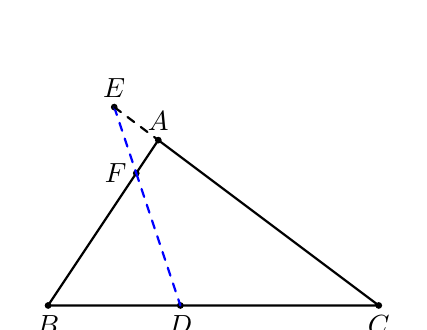
\begin{tikzpicture}[scale=0.7]
                \tkzDefPoint(0,3){A}
                \tkzDefPoint(-2,0){B}
                \tkzDefPoint(4,0){C}
                \coordinate (D) at ($(B)!0.4!(C)$);
                \coordinate (F) at ($(A)!0.2!(B)$);
                \tkzInterLL(D,F)(A,C) \tkzGetPoint{E}
                \tkzDrawPoints[fill=black](A,B,C,D,E,F)
                \tkzDrawPolygon[thick](A,B,C)
                \tkzDrawSegments[blue, thick, dashed](F,D E,F)
                \tkzDrawSegment[black, thick, dashed](E,A)
                \tkzLabelPoints[below](B,C,D)
                \tkzLabelPoints[above](A,E)
                \tkzLabelPoints[left](F)
            \end{tikzpicture}
            \caption{兩個內分點和一個外分點}
            \label{fig:coline_s1-1}
        \end{subfigure}
        \hfill % 在兩圖之間加入彈性間距
        \begin{subfigure}[b]{0.45\textwidth}
            \centering
            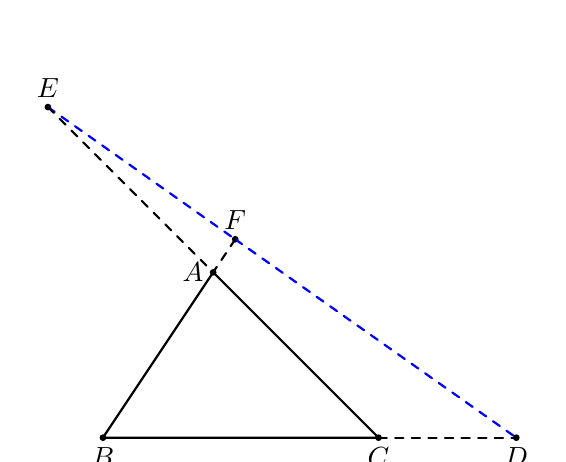
\begin{tikzpicture}[scale=0.7]
                 \tkzDefPoint(0,3){A}
                \tkzDefPoint(-2,0){B}
                \tkzDefPoint(3,0){C}
                \coordinate (D) at ($(B)!1.5!(C)$);
                \coordinate (F) at ($(A)!-0.2!(B)$);
                \tkzInterLL(D,F)(A,C) \tkzGetPoint{E}
                \tkzDrawPoints[fill=black](A,B,C,D,E,F)
                \tkzDrawPolygon[thick](A,B,C)
                \tkzDrawSegments[blue, thick, dashed](F,D E,F)
                \tkzDrawSegments[black, thick, dashed](E,A C,D F,A)
                \tkzLabelPoints[below](B,C,D)
                \tkzLabelPoints[above](E,F)
                \tkzLabelPoints[left](A)
                \end{tikzpicture}
            \caption{三個外分點}
            \label{fig:coline_s1-2}
        \end{subfigure}
    \end{figure}
\end{mybox}
\ifshow
\newpage
\begin{mybox}[必要性證明]{7em}{1em}{1em}
    方法一（Area Chasing）：以三角形的面積來表示各線段比值，並利用面積的加減關係證明定理。
    記$\triangle{XYZ}$的面積$[\triangle{XYZ}]$，則有：
    \begin{align}
        \frac{BD}{DC}&=\frac{[\triangle{EBD}]}{[\triangle{EDC}]}\label{eq:menalaus_BDDC}\\
        \frac{CE}{EA}&=\frac{[\triangle{EDC}]}{[\triangle{EAD}]}\label{eq:menalaus_CEEA}\\
        \frac{AF}{FB}&=\frac{[\triangle{EAF}]}{[\triangle{EFB}]}
        =\frac{[\triangle{DAF}]}{[\triangle{DFB}]}
        =\frac{[\triangle{EAF}]+[\triangle{DAF}]}{[\triangle{EFB}]+[\triangle{DFB}]}
        =\frac{[\triangle{EAD}]}{[\triangle{EBD}]}\label{eq:menalaus_AFFB}
    \end{align}
    把\eqref{eq:menalaus_BDDC}、\eqref{eq:menalaus_CEEA}和\eqref{eq:menalaus_AFFB}相乘，得：
    \begin{equation}
        \frac{BD}{DC}
        \cdot\frac{CE}{EA}
        \cdot\frac{AF}{FB}
        =\frac{[\triangle{EBD}]}{[\triangle{EDC}]}
        \cdot\frac{[\triangle{EDC}]}{[\triangle{EAD}]}
        \cdot\frac{[\triangle{EAD}]}{[\triangle{EBD}]}
        =1\label{eq:menalaus_novec}
    \end{equation}
    最後，因為一條直線與三角形三邊所在直線相交時，必定只會產生兩個內分點和一個外分點，或是三個外分點，
    所以
    \begin{equation}
        \frac{\overrightarrow{BD}}{\overrightarrow{DC}}
        \cdot\frac{\overrightarrow{CE}}{\overrightarrow{EA}}
        \cdot\frac{\overrightarrow{AF}}{\overrightarrow{FB}}
        =-\frac{BD}{DC}
        \cdot\frac{CE}{EA}
        \cdot\frac{AF}{FB}=-1\label{eq:menalaus_vec}
    \end{equation}
    由此證得梅涅勞斯定理的必要性。
\end{mybox}
\begin{mybox}[充分性證明]{7em}{1em}{1em}
    同一法：假設直線$DE$交直線$AB$於點$F'$，則由必要性可得：
    \[
        \frac{\overrightarrow{BD}}{\overrightarrow{DC}}
        \cdot\frac{\overrightarrow{CE}}{\overrightarrow{EA}}
        \cdot\frac{\overrightarrow{AF'}}{\overrightarrow{F'B}}=-1
    \]
    由充分性的已知條件，我們有：
    \[
        \frac{\overrightarrow{BD}}{\overrightarrow{DC}}
        \cdot\frac{\overrightarrow{CE}}{\overrightarrow{EA}}
        \cdot\frac{\overrightarrow{AF}}{\overrightarrow{FB}}=-1
    \]
    因此$F=F'$，即$D$、$E$、$F$三點共線，由此證得梅涅勞斯定理的充分性。
\end{mybox}
\newpage
\fi
\begin{mybox}[例題\thesection-1]{6em}{1em}{1em}
    在$\triangle{ABC}$中，$D$是邊$BC$上的點，滿足$BD:DC=1:2$；
    $E$是$CA$延長線上的點，滿足$CE:EA=3:1$。
    設$F$為直線$DE$與直線$AB$的交點，求$AF:FB$的值，並說明$F$是$AB$的外分點還是內分點。
    \stepcounter{figure}
    \begin{figure}[H]
        \centering 
        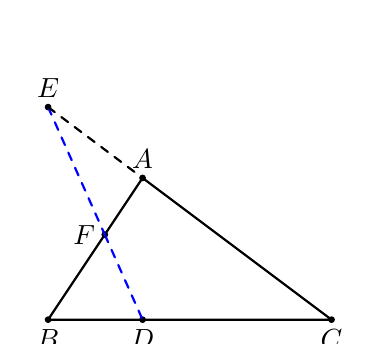
\begin{tikzpicture}[scale=0.6]
            \tkzDefPoint(0,3){A}
            \tkzDefPoint(-2,0){B}
            \tkzDefPoint(4,0){C}
            \coordinate (D) at ($(B)!1/3!(C)$);
            \coordinate (E) at ($(C)!1.5!(A)$);
            \tkzInterLL(D,E)(A,B) \tkzGetPoint{F}
            \tkzDrawPoints[fill=black](A,B,C,D,E,F)
            \tkzDrawPolygon[thick](A,B,C)
            \tkzDrawSegments[blue, thick, dashed](F,D E,F)
            \tkzDrawSegment[black, thick, dashed](E,A)
            \tkzLabelPoints[below](B,C,D)
            \tkzLabelPoints[above](A,E)
            \tkzLabelPoints[left](F)
        \end{tikzpicture}
        \caption{例題1-1示意圖}
        \label{fig:coline_s1-3}
    \end{figure}
\end{mybox}
\ifshow
\begin{mybox}[解]{3em}{1em}{1em}
根據梅涅勞斯定理：
    \[
        \frac{\overrightarrow{BD}}{\overrightarrow{DC}}
        \cdot\frac{\overrightarrow{CE}}{\overrightarrow{EA}}
        \cdot\frac{\overrightarrow{AF}}{\overrightarrow{FB}}=-1
    \]

    $D$在$BC$上，$BD:DC=1:2$，
    即$\overrightarrow{BD}/\overrightarrow{DC}=\frac{1}{2}$。

    $E$在$CA$延長線上，$CE:EA=3:2$，
    所以$\overrightarrow{CE}/\overrightarrow{EA}=-3$。

    代入梅涅勞斯定理：
    \begin{align*}
        &\frac{1}{2}\cdot\left(-3\right)
        \cdot\frac{\overrightarrow{AF}}{\overrightarrow{FB}}=-1\\
        \Leftrightarrow\quad&\frac{\overrightarrow{AF}}{\overrightarrow{FB}}=\frac{2}{3}
    \end{align*}
    因此$AF:FB=2:3$且$F$是$AB$的內分點。
\end{mybox}
\newpage
\fi
\begin{mybox}[例題\thesection-2]{6em}{1em}{1em}
    在 $\triangle ABC$ 中，點 $D$ 在邊 $BC$ 上，且滿足 $BD:DC = 2:1$。點 $E$ 是 $AC$ 邊的中點。連接 $AD$ 與 $BE$ 相交於點 $P$。
    \begin{enumerate}[label=(\roman*)]
        \item 求 $AP/PD$ 的比值。
        \item 求 $BP/PE$ 的比值。
    \end{enumerate}
    \begin{figure}[H]
        \centering 
        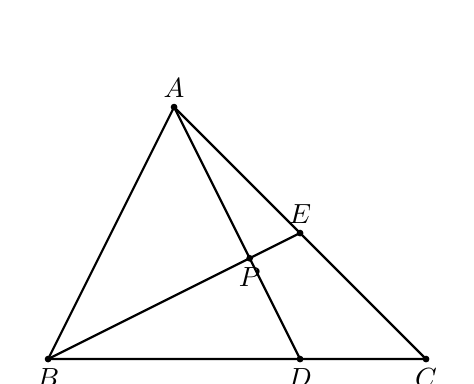
\begin{tikzpicture}[scale=0.8]
            \tkzDefPoint(0,4){A}
            \tkzDefPoint(-2,0){B}
            \tkzDefPoint(4,0){C}
            \coordinate (D) at ($(B)!2/3!(C)$);
            \coordinate (E) at ($(C)!0.5!(A)$);
            \tkzInterLL(A,D)(B,E) \tkzGetPoint{P}
            \tkzDrawPoints[fill=black](A,B,C,D,E,P)
            \tkzDrawPolygon[thick](A,B,C)
            \tkzDrawSegments[black, thick](A,D B,E)
            \tkzLabelPoints[below](B,C,D,P)
            \tkzLabelPoints[above](A,E)
        \end{tikzpicture}
        \caption{例題1-2示意圖}
        \label{fig:coline_s1-4}
    \end{figure}
\end{mybox}
\ifshow
\begin{mybox}[解]{3em}{0.5em}{1em}
此題給出了一個技巧——「需要求解 $XY/YZ$ 的比值，則需要觀察與$XYZ$相交的直線」。
\begin{enumerate}[label=(\roman*)]
    \item 觀察直線$BPE$，以這三點共線為切入點，使用梅涅勞斯定理：
    \begin{align*}
        &\frac{AP}{PD}\cdot\frac{DB}{BC}\cdot\frac{CE}{EA}=1\\
        \Leftrightarrow\quad&\frac{AP}{PD}\cdot\frac{2}{3}\cdot\frac{1}{1}=1\\
        \Leftrightarrow\quad&\frac{AP}{PD}=\frac{3}{2}
    \end{align*}
    \item 觀察直線$APD$，以這三點共線為切入點，使用梅涅勞斯定理：
    \begin{align*}
        &\frac{BP}{PE}\cdot\frac{EA}{AC}\cdot\frac{CD}{DB}=1\\
        \Leftrightarrow\quad&\frac{BP}{PE}\cdot\frac{1}{2}\cdot\frac{1}{2}=1\\
        \Leftrightarrow\quad&\frac{BP}{PE}=4
    \end{align*}
\end{enumerate}
\end{mybox}
\newpage
\fi
\begin{mybox}[例題\thesection-3]{6em}{1em}{1em}
    設 $AD$ 為 $\triangle ABC$ 內角 $\angle BAC$ 的平分線，$D$ 在 $BC$ 上。$E$ 為 $AC$ 中點。
    $K$在線段$AD$上，$AK>KD$。設$M$為$AD$中點。若滿足條件：$2AB \cdot KM = AC \cdot KD$，
    求證：$B$、$E$、$K$ 三點共線。
    \begin{figure}[H]
        \centering 
        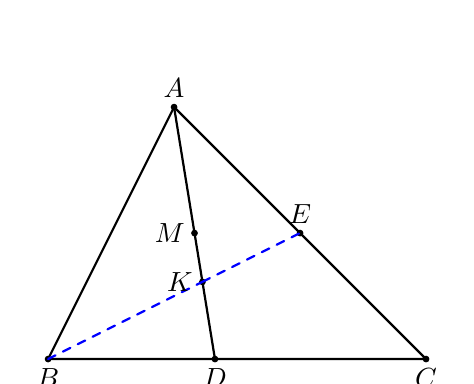
\begin{tikzpicture}[scale=0.8]
            \tkzDefPoint(0,4){A}
            \tkzDefPoint(-2,0){B}
            \tkzDefPoint(4,0){C}
            \tkzDefLine[bisector](B,A,C) \tkzGetPoint{D_tmp}
            \tkzInterLL(A,D_tmp)(B,C) \tkzGetPoint{D}
            %\coordinate (D) at ($(B)!1/3!(C)$);
            \coordinate (E) at ($(C)!0.5!(A)$);
            \coordinate (M) at ($(D)!0.5!(A)$);
            \tkzInterLL(B,E)(A,D) \tkzGetPoint{K}
            \tkzDrawPoints[fill=black](A,B,C,D,E,M,K)
            \tkzDrawPolygon[thick](A,B,C)
            \tkzDrawSegments[black, thick](A,D)
            \tkzDrawSegments[blue, thick, dashed](B,K K,E)
            \tkzLabelPoints[below](B,C,D)
            \tkzLabelPoints[above](A,E)
            \tkzLabelPoints[left](K,M)
        \end{tikzpicture}
        \caption{例題1-3示意圖}
        \label{fig:coline_s1-5}
    \end{figure}
\end{mybox}
\ifshow
\begin{mybox}[解]{3em}{1em}{1em}
    題目中的等式可等價變換為：
    \begin{align}
        &AB\cdot\left(AK-KD\right)=AC\cdot KD\notag\\
        \Leftrightarrow\quad&AB\cdot AK=KD\left(AB+AC\right)\notag\\
        \Leftrightarrow\quad&\frac{AK}{KD}=\frac{AB+AC}{AB}\label{eq:formula_1}
    \end{align}
    由角平分線定理可得：
    \begin{equation*}
        \frac{AB+AC}{AB}=\frac{BC}{BD}\label{eq:bisctor_theorem}
    \end{equation*}
    所以\eqref{eq:formula_1}等價於
    \begin{equation}
        \frac{AK}{KD}\cdot\frac{DB}{BC}=1\label{eq:formula_2}
    \end{equation}
    因為$E$是$AC$的中點，所以有
    \begin{equation*}
        \frac{AK}{KD}\cdot\frac{DB}{BC}\cdot\frac{CE}{EA}=1
    \end{equation*}
    根據梅涅勞斯定理可知$B$、$E$、$K$三點共線。
\end{mybox}
\fi
\newpage
\section{三線共點——塞瓦定理}
塞瓦定理是處理三線共點問題的強大工具，是把三線共點問題轉化為線段比值的乘積問題。與上一章的梅涅勞斯定理互為對偶。
\begin{mybox}[定理]{4em}{1em}{1em}
    給定$\triangle{ABC}$，若點$D$、$E$、$F$分別位於直線$BC$、$CA$、$AB$上，
    則$AD$、$BE$、$CF$三線共點的充分必要條件是：
    \begin{equation*}
        \frac{\overrightarrow{BD}}{\overrightarrow{DC}}
        \cdot\frac{\overrightarrow{CE}}{\overrightarrow{EA}}
        \cdot\frac{\overrightarrow{AF}}{\overrightarrow{FB}} = 1
    \end{equation*}
\end{mybox}
\ifshow
\begin{mybox}[必要性證明]{7em}{1em}{1em}
    \begin{center}
        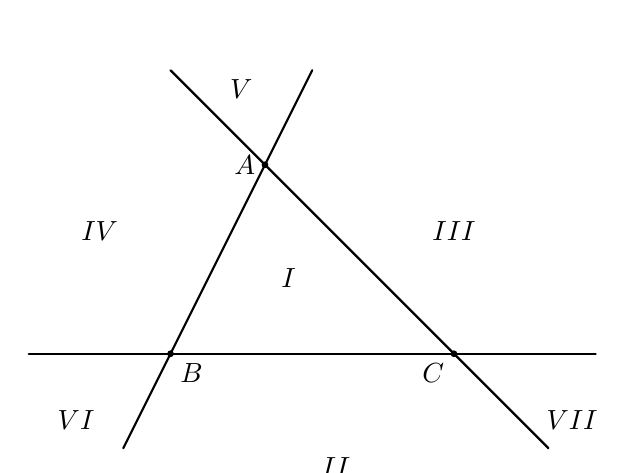
\begin{tikzpicture}[scale=0.6]
            \tkzDefPoint(0,4){A}
            \tkzDefPoint(-2,0){B}
            \tkzDefPoint(4,0){C}
            \tkzDrawLine[black, thick, add=0.5 and 0.5](A,B)
            \tkzDrawLine[black, thick, add=0.5 and 0.5](B,C)
            \tkzDrawLine[black, thick, add=0.5 and 0.5](C,A)
            \coordinate (D) at ($(B)!0.5!(C)$);
            \coordinate (E) at ($(C)!0.5!(A)$);
            \coordinate (F) at ($(A)!0.5!(B)$);
            \coordinate (I) at ($(D)!0.5!(A)$);

            \coordinate (II) at ($(D)!-0.5!(A)$);
            \coordinate (III) at ($(E)!-0.5!(B)$);
            \coordinate (IV) at ($(F)!-0.5!(C)$);
            \coordinate (V) at ($(D)!1.5!(A)$);             
            \coordinate (VI) at ($(E)!1.5!(B)$);
            \coordinate (VII) at ($(F)!1.5!(C)$); 
            \tkzDrawPoints[fill=black](A,B,C)
            \tkzLabelPoints[left](A)
            \tkzLabelPoints[below right](B)
            \tkzLabelPoints[below left](C)  
            \tkzLabelPoints(I,II,III,IV,V,VI,VII)
        \end{tikzpicture}
        \vspace{0.5cm}
        \noindent
        \begin{minipage}{\textwidth}
        \centering
        圖2-1\quad 平面分區示意圖
        \end{minipage}%
    \end{center}
    首先，三角形三邊所在直線將平面分成七個區域，如上圖所示。設$AD$、$BE$、$CF$三線交於點$P$，需要分別討論$P$位於不同區域的情況。（只須討論$I$、$II$、$V$區，其他區域可類推）
    \begin{enumerate}[label=Case \arabic*：, itemsep=2em]
        \item $P$位於$I$區
        \begin{center}
            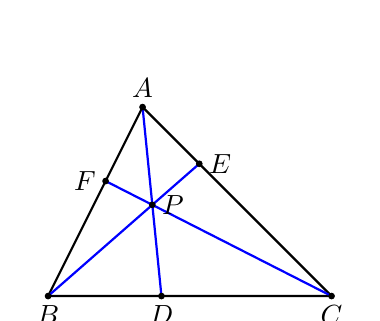
\begin{tikzpicture}[scale=0.6]
                \tkzDefPoint(0,4){A}
                \tkzDefPoint(-2,0){B}
                \tkzDefPoint(4,0){C}
                \coordinate (D) at ($(B)!0.4!(C)$);
                \coordinate (E) at ($(C)!0.7!(A)$);
                \tkzInterLL(A,D)(B,E) \tkzGetPoint{P}
                \tkzInterLL(C,P)(A,B) \tkzGetPoint{F}
                \tkzDrawPolygon[thick](A,B,C)
                \tkzDrawSegments[blue, thick](A,D B,E C,F)
                \tkzDrawPoints[fill=black](A,B,C,D,E,F,P)
                \tkzLabelPoints[above](A)
                \tkzLabelPoints[below](B,C,D)
                \tkzLabelPoints[right](E)
                \tkzLabelPoints[left](F)
                \tkzLabelPoints[right](P)
            \end{tikzpicture}
            \vspace{0.5cm}
            \noindent
            \begin{minipage}{\textwidth}
            \centering
            圖2-2\quad $P$位於$I$區的示意圖
            \end{minipage}%
        \end{center}
        此時，$D$、$E$、$F$均為內分點，根據燕尾定理可知：
        \begin{equation}
            \begin{cases}
                \overrightarrow{BD}/\overrightarrow{DC}=BD/DC=\left[\triangle{BPA}\right]/\left[\triangle{CPA}\right]\\
                \overrightarrow{CE}/\overrightarrow{EA}=CE/EA=\left[\triangle{CPB}\right]/\left[\triangle{APB}\right]\\
                \overrightarrow{AF}/\overrightarrow{FB}=AF/FB=\left[\triangle{APC}\right]/\left[\triangle{BPC}\right]
            \end{cases}\label{eq:ceva_case1-1}
        \end{equation}
        把\eqref{eq:ceva_case1-1}式三者相乘可得
        \begin{equation}
            \frac{\overrightarrow{BD}}{\overrightarrow{DC}}
            \cdot\frac{\overrightarrow{CE}}{\overrightarrow{EA}}
            \cdot\frac{\overrightarrow{AF}}{\overrightarrow{FB}}
            =\frac{\left[\triangle{BPA}\right]}{\left[\triangle{CPA}\right]}
            \cdot\frac{\left[\triangle{CPB}\right]}{\left[\triangle{APB}\right]}
            \cdot\frac{\left[\triangle{APC}\right]}{\left[\triangle{BPC}\right]}
            =1\label{eq:ceva_case1-2}
        \end{equation}

        \item $P$位於$II$區
        \begin{center}
            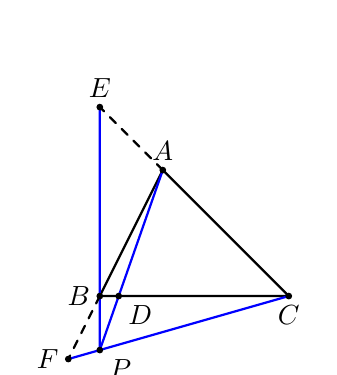
\begin{tikzpicture}[scale=0.4]
                \tkzDefPoint(0,4){A}
                \tkzDefPoint(-2,0){B}
                \tkzDefPoint(4,0){C}
                \coordinate (D) at ($(B)!0.1!(C)$);
                \coordinate (E) at ($(C)!1.5!(A)$);
                \tkzInterLL(A,D)(B,E) \tkzGetPoint{P}
                \tkzInterLL(C,P)(A,B) \tkzGetPoint{F}
                \tkzDrawPolygon[thick](A,B,C)
                \tkzDrawSegments[blue, thick](A,P P,E C,F)
                \tkzDrawSegments[black, thick, dashed](B,F A,E)
                \tkzDrawPoints[fill=black](A,B,C,D,E,F,P)
                \tkzLabelPoints[above](A,E)
                \tkzLabelPoints[below](C)
                \tkzLabelPoints[left](B,F)
                \tkzLabelPoints[below right](P,D)
            \end{tikzpicture}
            \vspace{0.5cm}
            \noindent
            \begin{minipage}{\textwidth}
            \centering
            圖2-3\quad $P$位於$II$區的示意圖
            \end{minipage}%
        \end{center}
        此時，$D$為內分點，$E$、$F$為外分點，根據燕尾定理可知：
        \begin{equation}
            \begin{cases}
                \overrightarrow{BD}/\overrightarrow{DC}=BD/DC=\left[\triangle{BPA}\right]/\left[\triangle{CPA}\right]\\
                \overrightarrow{CE}/\overrightarrow{EA}=-CE/EA=-\left[\triangle{CPB}\right]/\left[\triangle{APB}\right]\\
                \overrightarrow{AF}/\overrightarrow{FB}=-AF/FB=-\left[\triangle{APC}\right]/\left[\triangle{BPC}\right]
            \end{cases}\label{eq:ceva_case2-1}
        \end{equation}
        把\eqref{eq:ceva_case2-1}式三者相乘可得
        \begin{equation}
            \frac{\overrightarrow{BD}}{\overrightarrow{DC}}
            \cdot\frac{\overrightarrow{CE}}{\overrightarrow{EA}}
            \cdot\frac{\overrightarrow{AF}}{\overrightarrow{FB}}
            =\frac{\left[\triangle{BPA}\right]}{\left[\triangle{CPA}\right]}
            \cdot\left(-\frac{\left[\triangle{CPB}\right]}{\left[\triangle{APB}\right]}\right)
            \cdot\left(-\frac{\left[\triangle{APC}\right]}{\left[\triangle{BPC}\right]}\right)
            =1\label{eq:ceva_case2-2}
        \end{equation}

        \item $P$位於$V$區
        \begin{center}
            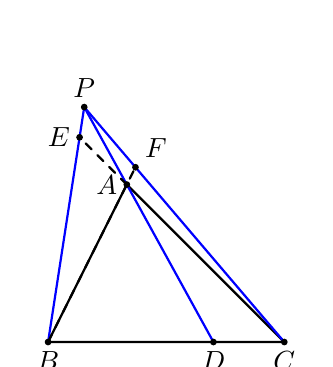
\begin{tikzpicture}[scale=0.5]
                \tkzDefPoint(0,4){A}
                \tkzDefPoint(-2,0){B}
                \tkzDefPoint(4,0){C}
                \coordinate (D) at ($(B)!0.7!(C)$);
                \coordinate (E) at ($(C)!1.3!(A)$);
                \tkzInterLL(A,D)(B,E) \tkzGetPoint{P}
                \tkzInterLL(C,P)(A,B) \tkzGetPoint{F}
                \tkzDrawPolygon[thick](A,B,C)
                \tkzDrawSegments[blue, thick](D,P B,P C,P)
                \tkzDrawSegments[black, thick, dashed](B,F A,E)
                \tkzDrawPoints[fill=black](A,B,C,D,E,F,P)
                \tkzLabelPoints[above](P)
                \tkzLabelPoints[below](B,C,D)
                \tkzLabelPoints[left](A,E)
                \tkzLabelPoints[above right](F)
            \end{tikzpicture}
            \vspace{0.5cm}
            \noindent
            \begin{minipage}{\textwidth}
            \centering
            圖2-3\quad $P$位於$V$區的示意圖
            \end{minipage}%
        \end{center}
        此時，$D$為內分點，$E$、$F$為外分點，根據燕尾定理可知：
        \begin{equation}
            \begin{cases}
                \overrightarrow{BD}/\overrightarrow{DC}=BD/DC=\left[\triangle{BPA}\right]/\left[\triangle{CPA}\right]\\
                \overrightarrow{CE}/\overrightarrow{EA}=-CE/EA=-\left[\triangle{CPB}\right]/\left[\triangle{APB}\right]\\
                \overrightarrow{AF}/\overrightarrow{FB}=-AF/FB=-\left[\triangle{APC}\right]/\left[\triangle{BPC}\right]
            \end{cases}\label{eq:ceva_case3-1}
        \end{equation}
        把\eqref{eq:ceva_case3-1}式三者相乘可得
        \begin{equation}
            \frac{\overrightarrow{BD}}{\overrightarrow{DC}}
            \cdot\frac{\overrightarrow{CE}}{\overrightarrow{EA}}
            \cdot\frac{\overrightarrow{AF}}{\overrightarrow{FB}}
            =\frac{\left[\triangle{BPA}\right]}{\left[\triangle{CPA}\right]}
            \cdot\left(-\frac{\left[\triangle{CPB}\right]}{\left[\triangle{APB}\right]}\right)
            \cdot\left(-\frac{\left[\triangle{APC}\right]}{\left[\triangle{BPC}\right]}\right)
            =1\label{eq:ceva_case3-2}
        \end{equation}
    \end{enumerate}
\end{mybox}
\begin{mybox}[充分性證明]{7em}{1em}{1em}
    同一法：假設直線$AD$交直線$BE$於點$P$，作直線$CP$交直線$AB$於點$F'$，則由必要性可得：
    \[
        \frac{\overrightarrow{BD}}{\overrightarrow{DC}}
        \cdot\frac{\overrightarrow{CE}}{\overrightarrow{EA}}
        \cdot\frac{\overrightarrow{AF'}}{\overrightarrow{F'B}} = 1
    \]
    由充分性的已知條件，我們有：
    \[
        \frac{\overrightarrow{BD}}{\overrightarrow{DC}}
        \cdot\frac{\overrightarrow{CE}}{\overrightarrow{EA}}
        \cdot\frac{\overrightarrow{AF}}{\overrightarrow{FB}}= 1
    \]
    因此$F=F'$，即$AD$、$BE$、$CF$三線共點，由此證得塞瓦定理的充分性。
\end{mybox}
\fi
\begin{mybox}[例題\thesection-1]{6em}{1em}{1em}
    求證：三角形三邊中線相交於一點。此點稱為三角形的「重心」。
\end{mybox}
\ifshow
\begin{mybox}[解]{3em}{1em}{1em}
    \begin{figure}[H]
        \centering 
        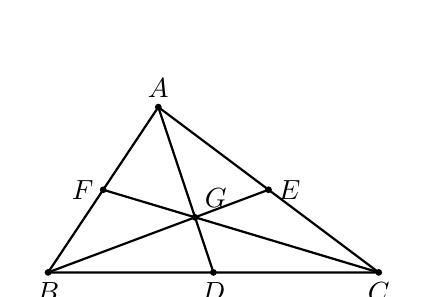
\begin{tikzpicture}[scale=0.7]
            \tkzDefPoint(0,3){A}
            \tkzDefPoint(-2,0){B}
            \tkzDefPoint(4,0){C}
            \coordinate (D) at ($(B)!0.5!(C)$);
            \coordinate (E) at ($(C)!0.5!(A)$);
            \coordinate (F) at ($(A)!0.5!(B)$);
            \tkzInterLL(A,D)(B,E) \tkzGetPoint{G}
            \tkzDrawPoints[fill=black](A,B,C,D,E,F,G)
            \tkzDrawPolygon[thick](A,B,C)
            \tkzDrawSegments[thick](A,D B,E C,F)
            \tkzLabelPoints[below](B,C,D)
            \tkzLabelPoints[above](A)
            \tkzLabelPoints[right](E)
            \tkzLabelPoints[left](F)
            \tkzLabelPoints[above right](G)
        \end{tikzpicture}
        \caption{例題2-1示意圖}
        \label{fig:coline_s2-1}
    \end{figure}
    對於任意$\triangle{ABC}$，$D$、$E$、$F$分別為邊$BC$、$CA$、$AB$的中點，則
    \begin{equation}
        \overrightarrow{BD}/\overrightarrow{DC}=\overrightarrow{CE}/\overrightarrow{EA}=\overrightarrow{AF}/\overrightarrow{FB}=1
    \end{equation}
    所以有
    \begin{equation}
        \frac{\overrightarrow{BD}}{\overrightarrow{DC}}
        \cdot\frac{\overrightarrow{CE}}{\overrightarrow{EA}}
        \cdot\frac{\overrightarrow{AF}}{\overrightarrow{FB}}=1\cdot 1\cdot 1=1
    \end{equation}
    由塞瓦定理可知，三條中線$AD$、$BE$、$CF$三線共點。
\end{mybox}
\fi
\begin{mybox}[例題 2.2]{6em}{1em}{1em}
    在 $\triangle ABC$ 中，$D$和$D'$為直線$BC$上兩個不同點，且$AD$和$AD'$分別為$\angle{BAC}$的內角平分線和外角平分線，$E$、$F$分別在直線$CA$、$AB$上。
    求證：$AD$、$BE$、$CF$三線共點的充分必要條件是$D'$、$E$、$F$三點共線。
    \begin{figure}[H]
        \centering 
        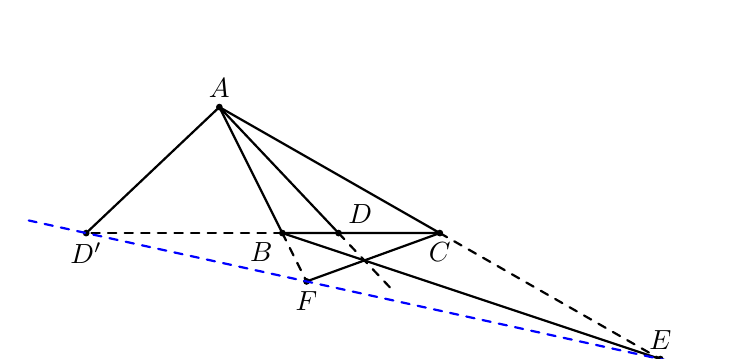
\begin{tikzpicture}[scale=0.4]
            \tkzDefPoint(-3,4){A}
            \tkzDefPoint(-1,0){B}
            \tkzDefPoint(4,0){C}
            \tkzDefLine[bisector](B,A,C) \tkzGetPoint{D_tmp}
            \tkzDefLine[bisector out](B,A,C) \tkzGetPoint{D'_tmp}
            \tkzInterLL(A,D_tmp)(B,C) \tkzGetPoint{D}
            \tkzInterLL(A,D'_tmp)(B,C) \tkzGetPoint{D'}
            \coordinate (E) at ($(C)!-1!(A)$);
            \tkzInterLL(D',E)(A,B) \tkzGetPoint{F}
            \tkzInterLL(B,E)(C,F) \tkzGetPoint{P}
            \tkzDrawPoints[fill=black](A,B,C,D,E,F,D')
            \tkzDrawPolygon[thick](A,B,C)
            \tkzDrawSegments[black, thick](A,D B,E C,F A,D')
            \tkzDrawSegments[black, thick, dashed](B,D' C,E B,F)
            \tkzLabelPoints[below](C,D',F)
            \tkzLabelPoints[above right](D)
            \tkzLabelPoints[below left](B)
            \tkzLabelPoints[above](A,E)
            \tkzDrawLine[black, thick, dashed, add=0 and 1](D,P)
            \tkzDrawLine[blue, thick, dashed, add=0.1 and 0.1](E,D')
        \end{tikzpicture}
        \caption{例題2-2示意圖}
        \label{fig:concurrent_s2-2}
    \end{figure}
\end{mybox}
\ifshow
\begin{mybox}[解]{3em}{1em}{1em}
    利用梅涅勞斯定理可知，$D'$、$E$、$F$三點共線的充分必要條件是：
    \begin{equation}
        \frac{\overrightarrow{BD'}}{\overrightarrow{D'C}}
        \cdot\frac{\overrightarrow{CE}}{\overrightarrow{EA}}
        \cdot\frac{\overrightarrow{AF}}{\overrightarrow{FB}} = -1\label{eq:ceva_example2-1}
    \end{equation}
    利用塞瓦定理可知，$AD$、$BE$、$CF$三線共點的充分必要條件是：
    \begin{equation}
        \frac{\overrightarrow{BD}}{\overrightarrow{DC}}
        \cdot\frac{\overrightarrow{CE}}{\overrightarrow{EA}}
        \cdot\frac{\overrightarrow{AF}}{\overrightarrow{FB}} = 1\label{eq:ceva_example2-2}
    \end{equation}
    因此原命題等價於證明
    \begin{equation}
        \frac{\overrightarrow{BD'}}{\overrightarrow{D'C}}=-\frac{\overrightarrow{BD}}{\overrightarrow{DC}}\label{eq:ceva_example2-3}
    \end{equation}
    \eqref{eq:ceva_example2-3}式可由角平分線定理證得。
\end{mybox}
\fi
\newpage
\section{三線共點——角元塞瓦定理}
角元塞瓦定理是另一個處理三線共點問題的工具，與塞瓦定理是等價的。此定理不依賴線段比值，而是依賴角度正弦比值。
\begin{mybox}[定理]{4em}{1em}{1em}
    給定$\triangle{ABC}$，$AD$、$BE$、$CF$三線共點的充分必要條件是：
    \begin{equation*}
        \frac{\sin{\measuredangle{BAD}}}{\sin{\measuredangle{DAC}}}
        \cdot\frac{\sin{\measuredangle{ACF}}}{\sin{\measuredangle{FCB}}}
        \cdot\frac{\sin{\measuredangle{CBE}}}{\sin{\measuredangle{ECA}}} = 1
    \end{equation*}
    此時不要求「$D$、$E$、$F$分別位於直線$BC$、$CA$、$AB$上」。
\end{mybox}
\ifshow
\begin{mybox}[證明]{4em}{1em}{1em}
    設直線$AD$交$BC$於$D'$，直線$BE$交$CA$於$E'$，直線$CF$交$AB$於$F'$。
    \begin{figure}[H]
        \centering
        \begin{subfigure}[b]{0.45\textwidth}
            \centering
            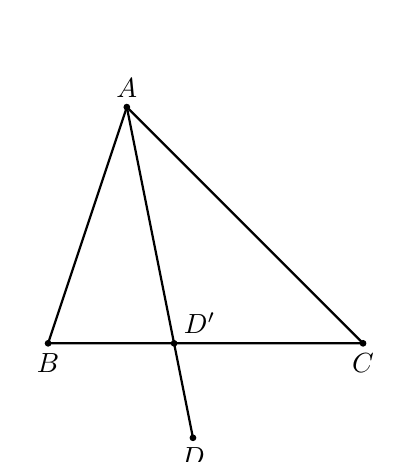
\begin{tikzpicture}
                \tkzDefPoints{0/0/A, -1/-3/B, 3/-3/C}
                \coordinate (D') at ($(B)!0.4!(C)$);
                \coordinate (D) at ($(A)!1.4!(D')$);
                \tkzDrawPolygon[black, thick](A,B,C)
                \tkzDrawSegments[black, thick](A,D)
                \tkzDrawPoints[fill=black](A,B,C,D,D')
                \tkzLabelPoints[above](A)
                \tkzLabelPoints[below](B,C,D)
                \tkzLabelPoints[above right](D')
            \end{tikzpicture}
            \caption{$D'$為$BC$的內分點}
            \label{fig:coline_s3-1}
        \end{subfigure}
        \hfill % 在兩圖之間加入彈性間距
        \begin{subfigure}[b]{0.45\textwidth}
            \centering
            \begin{tikzpicture}
                \tkzDefPoints{0/0/A, -1/-3/B, 3/-3/C}
                \coordinate (D') at ($(B)!1.4!(C)$);
                \coordinate (D) at ($(A)!1.4!(D')$);
                \tkzDrawPolygon[black, thick](A,B,C)
                \tkzDrawSegments[black, thick](A,D)
                \tkzDrawSegments[black, thick, dashed](C,D')
                \tkzDrawPoints[fill=black](A,B,C,D,D')
                \tkzLabelPoints[above](A)
                \tkzLabelPoints[below](B,C,D)
                \tkzLabelPoints[above right](D')
            \end{tikzpicture}
            \caption{$D'$為$BC$的外分點}
            \label{fig:coline_s3-2}
        \end{subfigure}
    \end{figure}
    利用正弦定理容易證得
    $$
        \frac{\sin{\measuredangle{BAD}}}{\sin{\measuredangle{DAC}}}=\frac{\overrightarrow{BD'}}{\overrightarrow{D'C}}\cdot\frac{CA}{AB}
    $$
    同理可得
    $$
        \frac{\sin{\measuredangle{ACF}}}{\sin{\measuredangle{FCB}}}=\frac{\overrightarrow{AF'}}{\overrightarrow{F'B}}\cdot\frac{BC}{CA}
    $$
    $$
        \frac{\sin{\measuredangle{CBE}}}{\sin{\measuredangle{EBA}}}=\frac{\overrightarrow{CE'}}{\overrightarrow{E'A}}\cdot\frac{AB}{BC}
    $$
    上面三式相乘可知
    \begin{equation*}
        \frac{\sin{\measuredangle{BAD}}}{\sin{\measuredangle{DAC}}}
        \cdot\frac{\sin{\measuredangle{ACF}}}{\sin{\measuredangle{FCB}}}
        \cdot\frac{\sin{\measuredangle{BCE}}}{\sin{\measuredangle{ECA}}}=\frac{\overrightarrow{BD'}}{\overrightarrow{D'C}}
        \cdot\frac{\overrightarrow{AF'}}{\overrightarrow{F'B}}
        \cdot\frac{\overrightarrow{CE'}}{\overrightarrow{E'A}}
    \end{equation*}
    結合塞瓦定理證得角元塞瓦定理。
\end{mybox}
\newpage
\fi
\begin{mybox}[例題\thesection-1]{6em}{1em}{1em}
    圓$\Omega$上按照順時針方向依次標出六點$A$、$B$、$C$、$D$、$E$、$F$。求證：直線$AD$、$BE$、$CF$三線共點的充分必要條件是：
    \begin{equation*}
        AB\cdot CD\cdot EF = AF\cdot BC\cdot DE
    \end{equation*}
\end{mybox}
\ifshow
\begin{mybox}[解]{3em}{1em}{1em}
    利用角元塞瓦定理可知，直線$AD$、$BE$、$CF$三線共點的充分必要條件是
    $$
        \frac{\sin{\measuredangle{DBE}}}{\sin{\measuredangle{EBF}}}
        \cdot\frac{\sin{\measuredangle{BFC}}}{\sin{\measuredangle{CFD}}}
        \cdot\frac{\sin{\measuredangle{FDA}}}{\sin{\measuredangle{ADB}}} = 1
    $$
    在圓$\Omega$上使用正弦定理可知
    $$
        \frac{DE}{EF}\cdot\frac{BC}{CD}\cdot\frac{FA}{AB}= 1
    $$
    即有 $AB\cdot CD\cdot EF = AF\cdot BC\cdot DE$。
\end{mybox}
\fi
\begin{mybox}[例題\thesection-2]{6em}{1em}{1em}
    對於$\triangle{ABC}$，記$AD$、$BE$、$CF$分別為$BC$、$CA$、$AB$邊上的中線。設$I$為$\triangle{ABC}$的內心，
    作$AD$關於$AI$的對稱直線$AD'$，$BE$關於$BI$的對稱直線$BE'$，$CF$關於$CI$的對稱直線$CF'$。
    
    求證：$AD'$、$BE'$、$CF'$三線共點。

    稱$AD'$、$BE'$、$CF'$分別為$BC$、$CA$、$AB$邊上的陪位中線，交點為陪位重心。
    \begin{figure}[H]
        \centering 
        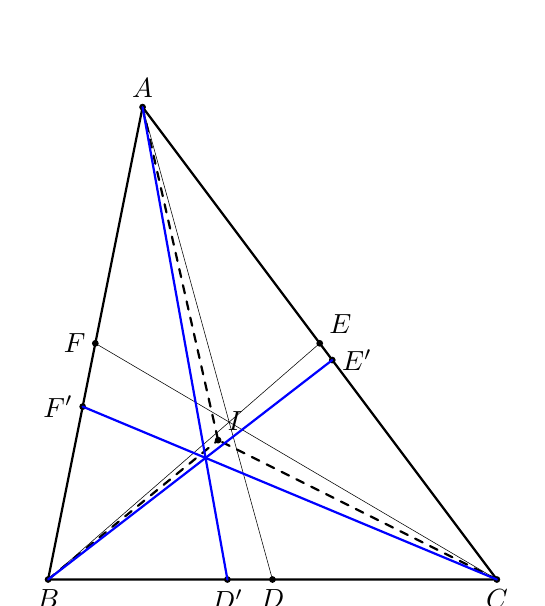
\begin{tikzpicture}[scale=0.6]
            \tkzDefPoints{0/10/A, -2/0/B, 7.5/0/C}
            \tkzDefTriangleCenter[in](A,B,C) \tkzGetPoint{I}
            \tkzDefTriangleCenter[centroid](A,B,C) \tkzGetPoint{G}
            \tkzInterLL(A,G)(B,C) \tkzGetPoint{D}
            \tkzInterLL(B,G)(C,A) \tkzGetPoint{E}
            \tkzInterLL(C,G)(A,B) \tkzGetPoint{F}
            \tkzDefPointsBy[reflection=over A--I](D){D'_tmp}
            \tkzDefPointsBy[reflection=over B--I](E){E'_tmp}
            \tkzDefPointsBy[reflection=over C--I](F){F'_tmp}
            \tkzInterLL(A,D'_tmp)(B,C) \tkzGetPoint{D'}
            \tkzInterLL(B,E'_tmp)(C,A) \tkzGetPoint{E'}
            \tkzInterLL(C,F'_tmp)(A,B) \tkzGetPoint{F'}
            \tkzDrawPoints[fill=black](A,B,C,D,E,F,I,D',E',F')
            \tkzDrawPolygon[black, thick](A,B,C)
            \tkzDrawSegments[black, thick, dashed](A,I B,I C,I)
            \tkzDrawSegments[black](A,D B,E C,F)
            \tkzDrawSegments[blue, thick](A,D' B,E' C,F')
            \tkzLabelPoints[above](A)
            \tkzLabelPoints[below](B,C,D,D')
            \tkzLabelPoints[left](F,F')
            \tkzLabelPoints[right](E')
            \tkzLabelPoints[above right](I,E)
        \end{tikzpicture}
        \caption{例題3-2示意圖}
        \label{fig:concurrent_s3-3}
    \end{figure}
\end{mybox}
\ifshow
\newpage
\begin{mybox}[解]{3em}{1em}{1em}
    易知$AD$、$BE$、$CF$三線共點（交點為$\triangle{ABC}$的重心），由角元塞瓦定理可知
    $$
        \frac{\sin{\measuredangle{BAD}}}{\sin{\measuredangle{DAC}}}
        \cdot\frac{\sin{\measuredangle{ACF}}}{\sin{\measuredangle{FCB}}}
        \cdot\frac{\sin{\measuredangle{CBE}}}{\sin{\measuredangle{ECA}}} = 1
    $$
    因為$AI$是$\angle{BAC}$的內角平分線，所以有
    $$
        \measuredangle{BAD'}=\measuredangle{DAC},\ \measuredangle{D'AC}=\measuredangle{BAD}
    $$
    即有
    $$
        \frac{\sin{\measuredangle{BAD'}}}{\sin{\measuredangle{D'AC}}}=\left(\frac{\sin{\measuredangle{BAD}}}{\sin{\measuredangle{DAC}}}\right)^{-1}
    $$
    同理可得
    $$
        \frac{\sin{\measuredangle{ACF'}}}{\sin{\measuredangle{F'CB}}}=\left(\frac{\sin{\measuredangle{ACF}}}{\sin{\measuredangle{FCB}}}\right)^{-1}
        \frac{\sin{\measuredangle{CBE'}}}{\sin{\measuredangle{E'CA}}}=\left(\frac{\sin{\measuredangle{CBE}}}{\sin{\measuredangle{ECA}}}\right)^{-1}
    $$
    因此
    $$
        \frac{\sin{\measuredangle{BAD'}}}{\sin{\measuredangle{D'AC}}}
        \cdot\frac{\sin{\measuredangle{ACF'}}}{\sin{\measuredangle{F'CB}}}
        \cdot\frac{\sin{\measuredangle{CBE'}}}{\sin{\measuredangle{E'CA}}}=\left(\frac{\sin{\measuredangle{BAD}}}{\sin{\measuredangle{DAC}}}
        \cdot\frac{\sin{\measuredangle{ACF}}}{\sin{\measuredangle{FCB}}}
        \cdot\frac{\sin{\measuredangle{CBE}}}{\sin{\measuredangle{ECA}}}\right)^{-1}=1
    $$
    由角元塞瓦定理可知，$AD'$、$BE'$、$CF'$三線共點。
\end{mybox}
\newpage
\fi
\section{練習題}
\begin{mybox}[Problem 1]{7em}{1em}{1em}
   求證：三角形三邊高線相交於一點。此點稱為三角形的「垂心」。
\end{mybox}
\begin{mybox}[Problem 2]{7em}{1em}{1em}
   給定$\triangle{ABC}$，$G$為$\triangle{ABC}$的重心，$M$為$BC$邊上的中點。求證：$AG/GM=2:1$。
\end{mybox}
\begin{mybox}[Problem 3]{7em}{1em}{1em}
   給定$\triangle{ABC}$中，$AD$、$BE$、$CF$分別為$\angle{BAC}$、$\angle{CBA}$、$\angle{ACB}$的外角平分線，
   且$D$、$E$、$F$分別位於直線$BC$、$CA$、$AB$上。求證：$D$、$E$、$F$三點共線。
\end{mybox}
\begin{mybox}[Problem 4]{7em}{1em}{1em}
   給定$\triangle{ABC}$中，$AD$、$BE$分別為$\angle{BAC}$、$\angle{CBA}$的內角平分線，$CF$為$\angle{ACB}$的外角平分線，
   且$D$、$E$、$F$分別位於直線$BC$、$CA$、$AB$上。求證：$D$、$E$、$F$三點共線。
\end{mybox}
\begin{mybox}[Problem 5]{7em}{1em}{1em}
   對於$\triangle{ABC}$，記$AD$、$BE$、$CF$分別為$BC$、$CA$、$AB$邊上的陪位中線。設$G'$為$\triangle{ABC}$的陪位重心。求證：
   $$
   \frac{AG'}{AD}+\frac{BG'}{BE}+\frac{CG'}{CF}=2
   $$
\end{mybox}
\begin{mybox}[Problem 6]{7em}{1em}{1em}
   給定$\triangle{ABC}$中，$AD$、$BE$分別為$\angle{BAC}$、$\angle{CBA}$的外角平分線，$CF$為$\angle{ACB}$的內角平分線，
   且$D$、$E$、$F$分別位於直線$BC$、$CA$、$AB$上。求證：$AD$、$BE$、$CF$三線共點。
\end{mybox}
\begin{mybox}[Problem 7]{7em}{1em}{1em}
   在$\triangle{ABC}$中，$D$和$E$分別為邊$AB$和$AC$上的點，滿足$DE\parallel BC$，記$BE$交$CD$與$P$，求證：直線$AP$平分邊$BC$。
\end{mybox}
\begin{mybox}[Problem 8]{7em}{1em}{1em}
   給定$\triangle{ABC}$中，邊$BC$、$CA$、$AB$上的中點分別為$P$、$Q$、$R$。
   $D$、$E$、$F$分別位於直線$BC$、$CA$、$AB$上，$D$、$E$、$F$分別關於$P$、$Q$、$R$的對稱點為$D'$、$E'$、$F'$。

   求證：
   \begin{enumerate}[label=(\roman*)]
       \item $AD$、$BE$、$CF$三線共點的充分必要條件是$AD'$、$BE'$、$CF'$三線共點。
       \item $D$、$E$、$F$三點共線的充分必要條件是$D'$、$E'$、$F'$三點共線。
   \end{enumerate}
\end{mybox}
\begin{mybox}[Problem 9]{7em}{1em}{1em}
   給定$\triangle{ABC}$中，$\angle{BAC}$、$\angle{CBA}$、$\angle{ACB}$上的內角平分線分別為$AP$、$BQ$、$CR$。
   $D$、$E$、$F$分別位於直線$BC$、$CA$、$AB$上，$AD$、$BE$、$CF$分別關於$AP$、$BQ$、$CR$的對稱直線為$AD'$、$BE'$、$CF'$。
   求證：$AD$、$BE$、$CF$三線共點的充分必要條件是$AD'$、$BE'$、$CF'$三線共點。
\end{mybox}
\begin{mybox}[Problem 10*]{7em}{1em}{1em}
    如下圖，$\triangle{ABC}$的內切圓分別切$BC$、$CA$、$AB$於點$D$、$E$、$F$，$P$為內切圓內的一點，
    線段$PA$、$PB$、$PC$分別與內切圓交於點$X$、$Y$、$Z$。
    
    證明：$XD$、$YE$、$ZF$三線共點。
    \begin{figure}[H]
        \centering 
        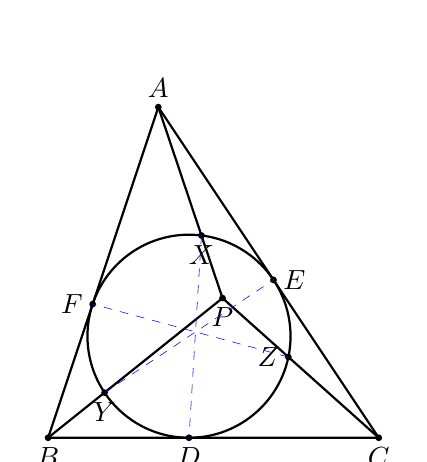
\begin{tikzpicture}[scale=0.7]
            \tkzDefPoint(0,6){A}
            \tkzDefPoint(-2,0){B}
            \tkzDefPoint(4,0){C}
            \tkzInCenter(A,B,C) \tkzGetPoint{I}
            \tkzDefPointBy[projection=onto B--C](I) \tkzGetPoint{D}
            \tkzDefPointBy[projection=onto C--A](I) \tkzGetPoint{E}
            \tkzDefPointBy[projection=onto A--B](I) \tkzGetPoint{F}
            \tkzDefPointBy[rotation=center I angle 15](E) \tkzGetPoint{E_tmp}
            \coordinate (P) at ($(I)!0.5!(E_tmp)$);
            \tkzInterLC(P,A)(I,D) \tkzGetPoints{X_tmp}{X}
            \tkzInterLC(P,B)(I,D) \tkzGetPoints{Y_tmp}{Y}
            \tkzInterLC(P,C)(I,D) \tkzGetPoints{Z}{Z_tmp}
            \tkzDrawPoints[fill=black](A,B,C,D,E,F,X,Y,Z,P)
            \tkzDrawPolygon[thick](A,B,C)
            \tkzDrawSegments[thick](P,A P,B P,C)
            \tkzLabelPoints[below](B,C,D,X,Y)
            \tkzLabelPoints[above](A)
            \tkzLabelPoints[right](E)
            \tkzLabelPoints[left](F,Z)
            \tkzLabelPoints[below](P)
            \tkzDrawCircle[black, thick](I,D)
            \tkzDrawSegments[blue, dashed](X,D Y,E Z,F)
        \end{tikzpicture}
        \caption{Problem 10*示意圖}
        \label{fig:p10}
    \end{figure}
\end{mybox}
\begin{mybox}[Problem 11*]{7em}{1em}{1em}
   在$\triangle{ABC}$中，$D$、$E$是邊$AB$、$AC$上的兩點，滿足$DE\parallel BC$。記$O_1$和$O_2$分別是$\triangle{ABE}$和$\triangle{ACD}$的外接圓圓心。
   直線$O_1O_2$分別交$AC$和$AB$於$P$和$Q$點。令$O$點是$\triangle{APQ}$的外接圓圓心，直線$AO$交$BC$於點$M$。
   
   求證：$M$為邊$BC$中點。
\end{mybox}
\end{document}